The proposed method's foundations rest on observation \ref{obs:observation_o}:

%%%%%%%%%%%%%%%%%%%%%%%%%%%%%%%%%%%%%%%%%%%%%%%%%%%%%%%%%%%%%%%%%%%%%%%%%%%%%%%%
\begin{customobs}{O}
  \label{obs:observation_o} It may be observed that there are conditions such
  that hypothesis \ref{hpt:hypothesis_h} stands true.
\end{customobs}

%%%%%%%%%%%%%%%%%%%%%%%%%%%%%%%%%%%%%%%%%%%%%%%%%%%%%%%%%%%%%%%%%%%%%%%%%%%%%%%%
\begin{customhpt}{H}
  \label{hpt:hypothesis_h}
  There exists $\overline{\delta} \in \mathbb{R}_{> 0}$ such that conjecture

\end{customhpt}

%%%%%%%%%%%%%%%%%%%%%%%%%%%%%%%%%%%%%%%%%%%%%%%%%%%%%%%%%%%%%%%%%%%%%%%%%%%%%%%%
\begin{customcnj}{C}
  %\label{hpt:hypothesis_h}
  \label{cnj:conjecture_c}
  Let the unknown pose of a 2D range sensor measuring range scan $\mathcal{S}_R$
  (def. \ref{def:definition_1}) be $\bm{p}(x,y,\theta)$ with respect to the
  reference frame of map $\bm{M}$.  Let $\mathcal{H}$ be a set of pose
  hypotheses within the free (i.e. traversable) space of $\bm{M}$:
  $\mathcal{H} = \{\hat{\bm{p}}_i(\hat{x}_i,\hat{y}_i,\hat{\theta}_i)\} \subseteq \texttt{free}(\bm{M})$, $i=0,1,\dots,|\mathcal{H}|-1$; $\mathbb{S}$
  be the set of map-scans (def. \ref{def:definition_2}) of $\bm{M}$ from pose
  hypotheses $\mathcal{H}$:
  $\mathbb{S} = \{\mathcal{S}_V^{\bm{M}}(\hat{\bm{p}}_i)\}$; and $\Psi$ be the
  set of CAERs (def. \ref{def:definition_3}) between $\mathcal{S}_R$ and the
  elements of $\mathbb{S}$:
  $\Psi = \{\psi(\mathcal{S}_R, \mathcal{S}_V^{\bm{M}}(\hat{\bm{p}}_i))\}$.
  Let $\mathcal{V} = \{\hat{\bm{p}}_i \in \mathcal{H}: \|\bm{p}-\hat{\bm{p}}_i\|_2 < \delta_0 \text{ and } \psi(\mathcal{S}_R,\mathcal{S}_V^{\bm{M}}(\hat{\bm{p}}_i)) < \psi_0\}$.
  Without loss of generality there exist $\delta_0$, $\overline{\delta}$, $\psi_0$ $\in \mathbb{R}_{> 0}$
  such that inequalities
  \begin{align}
    \delta_0 &< \overline{\delta} \nonumber \\
    \|\bm{p}-\hat{\bm{p}}_\mathcal{V}\|_2 &< \delta_0 \nonumber \\
    \psi(\mathcal{S}_R,\mathcal{S}_V^{\bm{M}}(\hat{\bm{p}}_\mathcal{V})) &< \psi_0 \nonumber
  \end{align}
  are simultaneously true for all $\hat{\bm{p}}_\mathcal{V} \in \mathcal{V}$,
  for which
  \begin{align}
    \psi(\bm{p}, \hat{\bm{p}}_\mathcal{V}) &< \psi(\bm{p}, \hat{\bm{p}}_{}) \ \ \ \Leftrightarrow \nonumber \\
    \|\bm{p}-\hat{\bm{p}}_\mathcal{V}\|_2 &< \|\bm{p}-\hat{\bm{p}}_{}\|_2 \nonumber
  \end{align}
  for any $\hat{\bm{p}}_{} \in {\mathcal{H} \setminus  \mathcal{V}}: \|\bm{p}-\hat{\bm{p}}_{}\|_2 \geq \delta_0$.
\end{customcnj}

%%%%%%%%%%%%%%%%%%%%%%%%%%%%%%%%%%%%%%%%%%%%%%%%%%%%%%%%%%%%%%%%%%%%%%%%%%%%%%%%
\begin{remark}
  \label{rem:remark_1}
  The composition of
  $\mathcal{H} = \mathcal{V} \cup \mathcal{X} \cup \mathcal{W}$, where
  $\mathcal{X} = \hat{\bm{p}} \in {\mathcal{H} \setminus \mathcal{V}}: \|\bm{p}-\hat{\bm{p}}\|_2 \geq \delta_0$ and
  $\mathcal{W} = \hat{\bm{p}} \in {\mathcal{H} \setminus \mathcal{V}}: \|\bm{p}-\hat{\bm{p}}\|_2 < \delta_0$.
  With respect to set $\mathcal{W}$ ... ??
\end{remark}


Figure \ref{fig:h_fig1} depicts a configuration which yields observation
\ref{obs:observation_o}, and where therefore hypothesis \ref{hpt:hypothesis_h}
is true.


\begin{figure}
  % GNUPLOT: LaTeX picture with Postscript
\begingroup
  \makeatletter
  \providecommand\color[2][]{%
    \GenericError{(gnuplot) \space\space\space\@spaces}{%
      Package color not loaded in conjunction with
      terminal option `colourtext'%
    }{See the gnuplot documentation for explanation.%
    }{Either use 'blacktext' in gnuplot or load the package
      color.sty in LaTeX.}%
    \renewcommand\color[2][]{}%
  }%
  \providecommand\includegraphics[2][]{%
    \GenericError{(gnuplot) \space\space\space\@spaces}{%
      Package graphicx or graphics not loaded%
    }{See the gnuplot documentation for explanation.%
    }{The gnuplot epslatex terminal needs graphicx.sty or graphics.sty.}%
    \renewcommand\includegraphics[2][]{}%
  }%
  \providecommand\rotatebox[2]{#2}%
  \@ifundefined{ifGPcolor}{%
    \newif\ifGPcolor
    \GPcolorfalse
  }{}%
  \@ifundefined{ifGPblacktext}{%
    \newif\ifGPblacktext
    \GPblacktexttrue
  }{}%
  % define a \g@addto@macro without @ in the name:
  \let\gplgaddtomacro\g@addto@macro
  % define empty templates for all commands taking text:
  \gdef\gplfronttext{}%
  \gdef\gplfronttext{}%
  \makeatother
  \ifGPblacktext
    % no textcolor at all
    \def\colorrgb#1{}%
    \def\colorgray#1{}%
  \else
    % gray or color?
    \ifGPcolor
      \def\colorrgb#1{\color[rgb]{#1}}%
      \def\colorgray#1{\color[gray]{#1}}%
      \expandafter\def\csname LTw\endcsname{\color{white}}%
      \expandafter\def\csname LTb\endcsname{\color{black}}%
      \expandafter\def\csname LTa\endcsname{\color{black}}%
      \expandafter\def\csname LT0\endcsname{\color[rgb]{1,0,0}}%
      \expandafter\def\csname LT1\endcsname{\color[rgb]{0,1,0}}%
      \expandafter\def\csname LT2\endcsname{\color[rgb]{0,0,1}}%
      \expandafter\def\csname LT3\endcsname{\color[rgb]{1,0,1}}%
      \expandafter\def\csname LT4\endcsname{\color[rgb]{0,1,1}}%
      \expandafter\def\csname LT5\endcsname{\color[rgb]{1,1,0}}%
      \expandafter\def\csname LT6\endcsname{\color[rgb]{0,0,0}}%
      \expandafter\def\csname LT7\endcsname{\color[rgb]{1,0.3,0}}%
      \expandafter\def\csname LT8\endcsname{\color[rgb]{0.5,0.5,0.5}}%
    \else
      % gray
      \def\colorrgb#1{\color{black}}%
      \def\colorgray#1{\color[gray]{#1}}%
      \expandafter\def\csname LTw\endcsname{\color{white}}%
      \expandafter\def\csname LTb\endcsname{\color{black}}%
      \expandafter\def\csname LTa\endcsname{\color{black}}%
      \expandafter\def\csname LT0\endcsname{\color{black}}%
      \expandafter\def\csname LT1\endcsname{\color{black}}%
      \expandafter\def\csname LT2\endcsname{\color{black}}%
      \expandafter\def\csname LT3\endcsname{\color{black}}%
      \expandafter\def\csname LT4\endcsname{\color{black}}%
      \expandafter\def\csname LT5\endcsname{\color{black}}%
      \expandafter\def\csname LT6\endcsname{\color{black}}%
      \expandafter\def\csname LT7\endcsname{\color{black}}%
      \expandafter\def\csname LT8\endcsname{\color{black}}%
    \fi
  \fi
    \setlength{\unitlength}{0.0500bp}%
    \ifx\gptboxheight\undefined%
      \newlength{\gptboxheight}%
      \newlength{\gptboxwidth}%
      \newsavebox{\gptboxtext}%
    \fi%
    \setlength{\fboxrule}{0.5pt}%
    \setlength{\fboxsep}{1pt}%
\begin{picture}(5000.00,5500.00)%
    \gplgaddtomacro\gplfronttext{%
      \colorrgb{0.15,0.15,0.15}%
      \put(368,3217){\makebox(0,0)[r]{\strut{}$0$}}%
      \colorrgb{0.15,0.15,0.15}%
      \put(368,3505){\makebox(0,0)[r]{\strut{}$c_0$}}%
      \colorrgb{0.15,0.15,0.15}%
      \put(368,3794){\makebox(0,0)[r]{\strut{}$400$}}%
      \colorrgb{0.15,0.15,0.15}%
      \put(368,4372){\makebox(0,0)[r]{\strut{}$800$}}%
      \colorrgb{0.15,0.15,0.15}%
      \put(368,4949){\makebox(0,0)[r]{\strut{}$1200$}}%
      \colorrgb{0.15,0.15,0.15}%
      \put(500,2997){\makebox(0,0){\strut{}$0$}}%
      \colorrgb{0.15,0.15,0.15}%
      \put(1100,2997){\makebox(0,0){\strut{}$\delta_0$}}%
      \colorrgb{0.15,0.15,0.15}%
      \put(1833,2997){\makebox(0,0){\strut{}$1.5$}}%
      \colorrgb{0.15,0.15,0.15}%
      \put(3166,2997){\makebox(0,0){\strut{}$3$}}%
      \colorrgb{0.15,0.15,0.15}%
      \put(4499,2997){\makebox(0,0){\strut{}$4.5$}}%
    }%
    \gplgaddtomacro\gplfronttext{%
      \colorrgb{0.15,0.15,0.15}%
      \put(-402,4083){\rotatebox{90}{\makebox(0,0){\strut{}CAER [m]}}}%
      \colorrgb{0.15,0.15,0.15}%
      \put(2499,2667){\makebox(0,0){\strut{}pose estimate error [(m$^2$ + rad$^2$)$^{1/2}$]}}%
      \put(1013,3330){\makebox(0,0){$\mathcal{V}$}}%
      \put(2600,4000){\makebox(0,0){\color{white}$\hat{\bm{p}} \in \mathcal{H} \backslash \mathcal{V} : \|\bm{p}-\hat{\bm{p}}\|_2 \geq \delta_0$}}%
    }%
    \gplgaddtomacro\gplfronttext{%
      \colorrgb{0.15,0.15,0.15}%
      \put(368,550){\makebox(0,0)[r]{\strut{}$0$}}%
      \colorrgb{0.15,0.15,0.15}%
      \put(368,810){\makebox(0,0)[r]{\strut{}$\delta_0$}}%
      \colorrgb{0.15,0.15,0.15}%
      \put(368,1127){\makebox(0,0)[r]{\strut{}$1.5$}}%
      \colorrgb{0.15,0.15,0.15}%
      \put(368,1705){\makebox(0,0)[r]{\strut{}$3.0$}}%
      \colorrgb{0.15,0.15,0.15}%
      \put(368,2282){\makebox(0,0)[r]{\strut{}$4.5$}}%
      \colorrgb{0.15,0.15,0.15}%
      \put(1300,330){\makebox(0,0){\strut{}$10^1$}}%
      \colorrgb{0.15,0.15,0.15}%
      \put(2100,330){\makebox(0,0){\strut{}$10^2$}}%
      \colorrgb{0.15,0.15,0.15}%
      \put(2899,330){\makebox(0,0){\strut{}$10^3$}}%
      \colorrgb{0.15,0.15,0.15}%
      \put(3699,330){\makebox(0,0){\strut{}$10^4$}}%
      \colorrgb{0.15,0.15,0.15}%
      \put(4499,330){\makebox(0,0){\strut{}$10^5$}}%
    }%
    \gplgaddtomacro\gplfronttext{%
      \colorrgb{0.15,0.15,0.15}%
      \put(-1194,1416){\rotatebox{90}{\makebox(0,0){\strut{}pose estimate error [(m$^2$ + rad$^2$)$^{1/2}$]}}}%
      \colorrgb{0.15,0.15,0.15}%
      \put(2499,0){\makebox(0,0){\strut{}position in ascending CAER hierarchy}}%
    }%
    \put(0,0){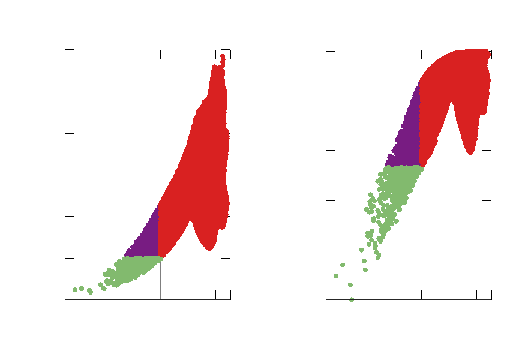
\includegraphics{./figures/h_fig}}%
    \gplfronttext
  \end{picture}%
\endgroup

  \vspace{1cm}
  \caption{\small }
  \label{fig:h_fig1}
\end{figure}

\begin{figure}[]\centering
  


\tikzset{every picture/.style={line width=0.75pt}} %set default line width to 0.75pt

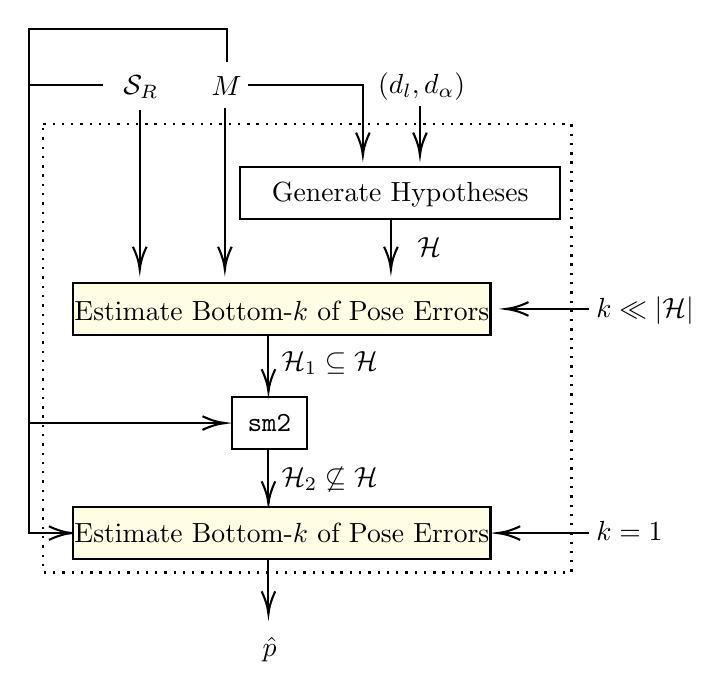
\begin{tikzpicture}[x=0.75pt,y=0.75pt,yscale=-1,xscale=1]
%uncomment if require: \path (0,412); %set diagram left start at 0, and has height of 412

%Shape: Rectangle [id:dp9638758944798029]
\draw  [dash pattern={on 0.84pt off 2.51pt}] (132,113) -- (386.5,113) -- (386.5,329) -- (132,329) -- cycle ;
%Straight Lines [id:da7180108526379969]
\draw    (178.5,106) -- (178.5,183) ;
\draw [shift={(178.5,183)}, rotate = 270] [color={rgb, 255:red, 0; green, 0; blue, 0 }  ][line width=0.75]    (10.93,-3.29) .. controls (6.95,-1.4) and (3.31,-0.3) .. (0,0) .. controls (3.31,0.3) and (6.95,1.4) .. (10.93,3.29)   ;
%Straight Lines [id:da03009202516620957]
\draw    (299.5,158) -- (299.5,183) ;
\draw [shift={(299.5,183)}, rotate = 270] [color={rgb, 255:red, 0; green, 0; blue, 0 }  ][line width=0.75]    (10.93,-3.29) .. controls (6.95,-1.4) and (3.31,-0.3) .. (0,0) .. controls (3.31,0.3) and (6.95,1.4) .. (10.93,3.29)   ;
%Straight Lines [id:da8319074018571286]
\draw    (219.5,105.33) -- (219.5,183) ;
\draw [shift={(219.5,183)}, rotate = 270] [color={rgb, 255:red, 0; green, 0; blue, 0 }  ][line width=0.75]    (10.93,-3.29) .. controls (6.95,-1.4) and (3.31,-0.3) .. (0,0) .. controls (3.31,0.3) and (6.95,1.4) .. (10.93,3.29)   ;
%Straight Lines [id:da9443063587697282]
\draw    (313.5,104) -- (313.5,125) ;
\draw [shift={(313.5,128)}, rotate = 270] [color={rgb, 255:red, 0; green, 0; blue, 0 }  ][line width=0.75]    (10.93,-3.29) .. controls (6.95,-1.4) and (3.31,-0.3) .. (0,0) .. controls (3.31,0.3) and (6.95,1.4) .. (10.93,3.29)   ;

%Straight Lines [id:da7873103370093042]
\draw    (230.79,94.31) -- (286,94.31) -- (286,125) ;
\draw [shift={(286,128)}, rotate = 270] [color={rgb, 255:red, 0; green, 0; blue, 0 }  ][line width=0.75]    (10.93,-3.29) .. controls (6.95,-1.4) and (3.31,-0.3) .. (0,0) .. controls (3.31,0.3) and (6.95,1.4) .. (10.93,3.29)   ;


%Straight Lines [id:da8514300443018634]
\draw    (160.79,94.31) -- (125,94.31) -- (125,257) -- (217.67,257) ;
\draw [shift={(219.67,257)}, rotate = 180] [color={rgb, 255:red, 0; green, 0; blue, 0 }  ][line width=0.75]    (10.93,-3.29) .. controls (6.95,-1.4) and (3.31,-0.3) .. (0,0) .. controls (3.31,0.3) and (6.95,1.4) .. (10.93,3.29)   ;
%Straight Lines [id:da6607120070694932]
\draw    (220.33,83.17) -- (220.33,67) -- (125,67) -- (125,94.31) ;
%Straight Lines [id:da5274799303628721]
\draw    (240.5,215) -- (240.5,240) ;
\draw [shift={(240.5,242)}, rotate = 270] [color={rgb, 255:red, 0; green, 0; blue, 0 }  ][line width=0.75]    (10.93,-3.29) .. controls (6.95,-1.4) and (3.31,-0.3) .. (0,0) .. controls (3.31,0.3) and (6.95,1.4) .. (10.93,3.29)   ;
%Straight Lines [id:da12312420020821957]
\draw    (395,202) -- (356.85,202) ;
\draw [shift={(354.85,202.01)}] [color={rgb, 255:red, 0; green, 0; blue, 0 }  ][line width=0.75]    (10.93,-3.29) .. controls (6.95,-1.4) and (3.31,-0.3) .. (0,0) .. controls (3.31,0.3) and (6.95,1.4) .. (10.93,3.29)   ;
%Straight Lines [id:da5566859790391938]
\draw    (240.5,269) -- (240.5,294) ;
\draw [shift={(240.5,296)}, rotate = 270] [color={rgb, 255:red, 0; green, 0; blue, 0 }  ][line width=0.75]    (10.93,-3.29) .. controls (6.95,-1.4) and (3.31,-0.3) .. (0,0) .. controls (3.31,0.3) and (6.95,1.4) .. (10.93,3.29)   ;
%Straight Lines [id:da8040278693931917]
\draw    (395,310) -- (352.85,310) ;
\draw [shift={(350.85,310)}] [color={rgb, 255:red, 0; green, 0; blue, 0 }  ][line width=0.75]    (10.93,-3.29) .. controls (6.95,-1.4) and (3.31,-0.3) .. (0,0) .. controls (3.31,0.3) and (6.95,1.4) .. (10.93,3.29)   ;
%Straight Lines [id:da30367866946140687]
\draw    (125,257) -- (125,310) -- (145.67,310) ;
\draw [shift={(145.67,310)}, rotate = 180] [color={rgb, 255:red, 0; green, 0; blue, 0 }  ][line width=0.75]    (10.93,-3.29) .. controls (6.95,-1.4) and (3.31,-0.3) .. (0,0) .. controls (3.31,0.3) and (6.95,1.4) .. (10.93,3.29)   ;
%Straight Lines [id:da9956825870606303]
\draw    (240.5,322) -- (240.5,347) ;
\draw [shift={(240.5,349)}, rotate = 270] [color={rgb, 255:red, 0; green, 0; blue, 0 }  ][line width=0.75]    (10.93,-3.29) .. controls (6.95,-1.4) and (3.31,-0.3) .. (0,0) .. controls (3.31,0.3) and (6.95,1.4) .. (10.93,3.29)   ;

% Text Node
\draw (179,95) node   [align=left] {$\mathcal{S}_R$};
% Text Node
\draw    (227,133.5) -- (381,133.5) -- (381,158.5) -- (227,158.5) -- cycle  ;
\draw (304,147) node   [align=left] {Generate Hypotheses};
% Text Node
\draw (318,172) node   [align=left] {$\mathcal{H}$};
% Text Node
\draw (220.33,94.83) node   [align=left] {$\bm{M}$};
% Text Node
% \draw (314.33,94.83) node   [align=left] {$|\mathcal{H}|$};
\draw (314.33,94.83) node   [align=left] {$(d_{\bm{l}}, d_{\alpha})$};
% Text Node
\draw    (223,244.5) -- (259,244.5) -- (259,269.5) -- (223,269.5) -- cycle  ;
\draw (241,257) node   [align=left] {\texttt{sm2}};
% Text Node
\draw  [fill={rgb, 255:red, 255; green, 254; blue, 229 }  ,fill opacity=1 ]  (146.5,189.5) -- (347.5,189.5) -- (347.5,214.5) -- (146.5,214.5) -- cycle  ;
\draw (247,203) node   [align=left] {Estimate Bottom-$k$ of Pose Errors};
% Text Node
\draw (397,194.71) node [anchor=north west][inner sep=0.75pt]   [align=left] {$k \ll |\mathcal{H}|$};
% Text Node
\draw  [fill={rgb, 255:red, 255; green, 254; blue, 229 }  ,fill opacity=1 ]  (146.5,297.5) -- (347.5,297.5) -- (347.5,322.5) -- (146.5,322.5) -- cycle  ;
\draw (247,310) node   [align=left] {Estimate Bottom-$k$ of Pose Errors};
% Text Node
\draw (397,302.71) node [anchor=north west][inner sep=0.75pt]   [align=left] {$k = 1$};
% Text Node
\draw (270,228) node   [align=left] {$\mathcal{H}_1 \subseteq \mathcal{H}$};
% Text Node
\draw (270,284) node   [align=left] {$\mathcal{H}_2 \not\subseteq \mathcal{H}$};
% Text Node
\draw (241,366) node   [align=left] {$\hat{\bm{p}}$};


\end{tikzpicture}

  \caption{\small }
  \label{fig:cbgl}
\end{figure}


\begin{figure}[]\centering
  

\tikzset{every picture/.style={line width=0.75pt}} %set default line width to 0.75pt

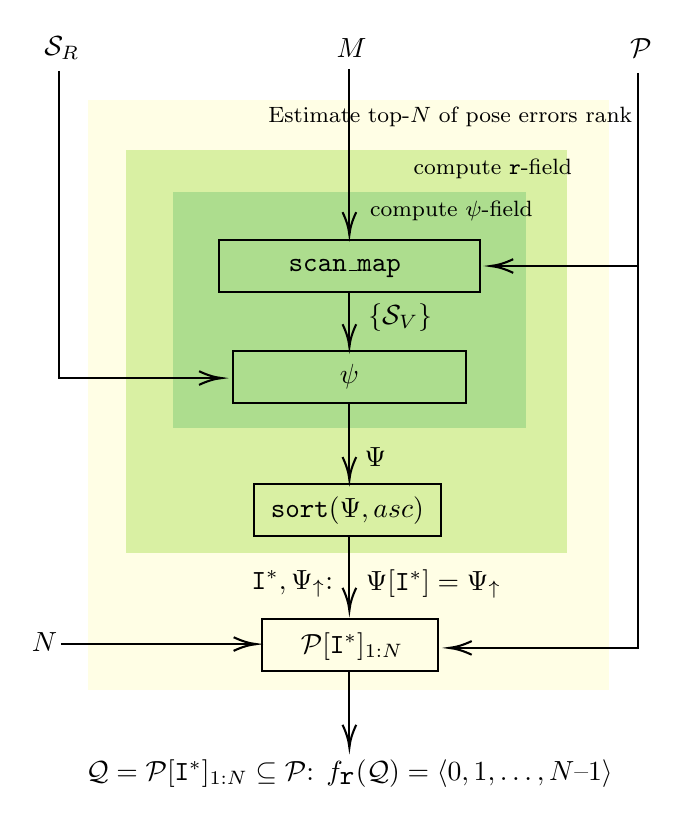
\begin{tikzpicture}[x=0.75pt,y=0.75pt,yscale=-1,xscale=1]
%uncomment if require: \path (0,561); %set diagram left start at 0, and has height of 561

%Shape: Rectangle [id:dp5322819707523847]
\draw  [draw opacity=0][fill={rgb, 255:red, 255; green, 254; blue, 229 }  ,fill opacity=1 ] (149.5,52) -- (400.5,52) -- (400.5,336) -- (149.5,336) -- cycle ;
%Shape: Rectangle [id:dp7467881383910988]
\draw  [draw opacity=0][fill={rgb, 255:red, 217; green, 240; blue, 163 }  ,fill opacity=1 ][dash pattern={on 4.5pt off 4.5pt}] (168,76) -- (380.5,76) -- (380.5,270) -- (168,270) -- cycle ;
%Shape: Rectangle [id:dp8406662160759257]
\draw  [draw opacity=0][fill={rgb, 255:red, 173; green, 221; blue, 142 }  ,fill opacity=1 ][dash pattern={on 0.84pt off 2.51pt}] (190.5,96) -- (360.5,96) -- (360.5,210) -- (190.5,210) -- cycle ;
%Straight Lines [id:da7895938434263794]
\draw    (135.5,37.83) -- (135.5,185.83) -- (212,185.83) ;
\draw [shift={(214,185.83)}, rotate = 180.12] [color={rgb, 255:red, 0; green, 0; blue, 0 }  ][line width=0.75]    (10.93,-3.29) .. controls (6.95,-1.4) and (3.31,-0.3) .. (0,0) .. controls (3.31,0.3) and (6.95,1.4) .. (10.93,3.29)   ;
%Straight Lines [id:da7692323493003017]
\draw    (275.5,36.83) -- (275.5,114.83) ;
\draw [shift={(275.5,116.83)}, rotate = 270] [color={rgb, 255:red, 0; green, 0; blue, 0 }  ][line width=0.75]    (10.93,-3.29) .. controls (6.95,-1.4) and (3.31,-0.3) .. (0,0) .. controls (3.31,0.3) and (6.95,1.4) .. (10.93,3.29)   ;
%Straight Lines [id:da7299087017419263]
\draw    (275.5,143.83) -- (275.5,168.83) ;
\draw [shift={(275.5,170.83)}, rotate = 270] [color={rgb, 255:red, 0; green, 0; blue, 0 }  ][line width=0.75]    (10.93,-3.29) .. controls (6.95,-1.4) and (3.31,-0.3) .. (0,0) .. controls (3.31,0.3) and (6.95,1.4) .. (10.93,3.29)   ;
%Straight Lines [id:da7271584666245074]
\draw    (275.5,326.83) -- (275.5,361.83) ;
\draw [shift={(275.5,363.83)}, rotate = 270] [color={rgb, 255:red, 0; green, 0; blue, 0 }  ][line width=0.75]    (10.93,-3.29) .. controls (6.95,-1.4) and (3.31,-0.3) .. (0,0) .. controls (3.31,0.3) and (6.95,1.4) .. (10.93,3.29)   ;
%Straight Lines [id:da28696405299112593]
\draw    (414.5,38.83) -- (414.5,131.83) -- (345.5,131.83) ;
\draw [shift={(343.5,131.83)}, rotate = 360] [color={rgb, 255:red, 0; green, 0; blue, 0 }  ][line width=0.75]    (10.93,-3.29) .. controls (6.95,-1.4) and (3.31,-0.3) .. (0,0) .. controls (3.31,0.3) and (6.95,1.4) .. (10.93,3.29)   ;
%Straight Lines [id:da6509243873520767]
\draw    (414.5,113.83) -- (414.5,315.83) -- (325.5,315.83) ;
\draw [shift={(323.5,315.83)}, rotate = 360] [color={rgb, 255:red, 0; green, 0; blue, 0 }  ][line width=0.75]    (10.93,-3.29) .. controls (6.95,-1.4) and (3.31,-0.3) .. (0,0) .. controls (3.31,0.3) and (6.95,1.4) .. (10.93,3.29)   ;
%Straight Lines [id:da2836399375619547]
\draw    (275.5,197.83) -- (275.5,232.83) ;
\draw [shift={(275.5,234.83)}, rotate = 270] [color={rgb, 255:red, 0; green, 0; blue, 0 }  ][line width=0.75]    (10.93,-3.29) .. controls (6.95,-1.4) and (3.31,-0.3) .. (0,0) .. controls (3.31,0.3) and (6.95,1.4) .. (10.93,3.29)   ;
%Straight Lines [id:da4366145475662475]
\draw    (136.52,314) -- (228.67,314) ;
\draw [shift={(230.67,314)}, rotate = 180.19] [color={rgb, 255:red, 0; green, 0; blue, 0 }  ][line width=0.75]    (10.93,-3.29) .. controls (6.95,-1.4) and (3.31,-0.3) .. (0,0) .. controls (3.31,0.3) and (6.95,1.4) .. (10.93,3.29)   ;
%Straight Lines [id:da01419967829423241]
\draw    (275.5,261.83) -- (275.5,295.83) ;
\draw [shift={(275.5,297.83)}, rotate = 270] [color={rgb, 255:red, 0; green, 0; blue, 0 }  ][line width=0.75]    (10.93,-3.29) .. controls (6.95,-1.4) and (3.31,-0.3) .. (0,0) .. controls (3.31,0.3) and (6.95,1.4) .. (10.93,3.29)   ;

% Text Node
\draw (235,54) node [anchor=north west][inner sep=0.75pt]   [align=left] {\footnotesize Estimate top-$N$ of pose errors rank};
\draw (305,79) node [anchor=north west][inner sep=0.75pt]   [align=left] {\footnotesize compute \texttt{r}-field};
\draw (284,99) node [anchor=north west][inner sep=0.75pt]   [align=left] {\footnotesize compute $\psi$-field};
% Text Node
\draw (137,27) node     [align=left] {$\mathcal{S}_R$};
\draw (276.5,27) node   [align=left] {$\bm{M}$};
\draw (416,27) node  [align=left] {$\mathcal{P}$};
% Text Node
\draw    (212.5,119.33) -- (338.5,119.33) -- (338.5,144.33) -- (212.5,144.33) -- cycle  ;
\draw (275.5,133) node   [align=left] { \ \ \ \ \ \texttt{scan\_map} \ \ \ \ \ };
% Text Node
\draw (300,156.83) node   [align=left] {$\{\mathcal{S}_V\}$};
% Text Node
\draw    (219.5,172.67) -- (331.5,172.67) -- (331.5,197.67) -- (219.5,197.67) -- cycle  ;
\draw (275.5,185.17) node   [align=left] { \ \ \ \ \ \ \ $\psi$ \ \ \ \ \ \ };
% Text Node
\draw    (229.5,237) -- (319.5,237) -- (319.5,262) -- (229.5,262) -- cycle  ;
\draw (274.5,249.5) node   [align=left] {$\texttt{sort}(\Psi,\text{asc})$};
% Text Node
\draw (288,224) node   [align=left] {$\Psi$};
% Text Node
% Text Node
% Text Node
% Text Node
\draw    (233.25,302) -- (318.25,302) -- (318.25,327) -- (233.25,327) -- cycle  ;
% Text Node
\draw (251,285) node   [align=left] {$\texttt{I}^{\ast}, \Psi_{\uparrow}$: };
\draw (316,285) node   [align=left] {$\Psi[\texttt{I}^{\ast}] = \Psi_{\uparrow}$};

\draw (276.75,315) node   [align=left] { $\mathcal{P}[\texttt{I}^{\ast}]_{1:N} $};
\draw (121,307) node [anchor=north west][inner sep=0.75pt]   [align=left] {$N$};
\draw (275.5,376.5) node   [align=left] {$\mathcal{Q} = \mathcal{P}[\texttt{I}^{\ast}]_{1:N} \subseteq \mathcal{P}$:
  $f_{\texttt{r}}(\mathcal{Q}) = \langle 0,1,\dots,N$--$1 \rangle$};

\end{tikzpicture}






  \caption{\small }
  \label{fig:cbgl}
\end{figure}





%% CBGL %%%%%%%%%%%%%%%%%%%%%%%%%%%%%%%%%%%%%%%%%%%%%%%%%%%%%%%%%%%%%%%%%%%%%%%%
\floatstyle{spaceruled}
\restylefloat{algorithm}
\begin{algorithm}
  \caption{\texttt{CBGL}}
  \begin{spacing}{1.2}
  \begin{algorithmic}[1]
    \REQUIRE $\mathcal{S}_R$, $\bm{M}$, $|\mathcal{H}|$, $\nabla$
    \ENSURE $\hat{\bm{p}}$
    \STATE $\mathcal{H} \leftarrow \{\varnothing\}$
    \FOR {$i \leftarrow 0,1,\dots,|\mathcal{H}|-1$}
      \STATE $\hat{\bm{p}}_i \leftarrow \texttt{rand}(\hat{x},\hat{y},\hat{\theta}): (x,y) \in \texttt{free}(\bm{M})$
      \STATE $\mathcal{H} \leftarrow \{\mathcal{H}, \hat{\bm{p}}_i\}$
    \ENDFOR
    \STATE $\mathcal{H}_1 \leftarrow$ \texttt{bottom}$\_n\_\texttt{poses}(\mathcal{S}_R, \bm{M}, \mathcal{H}, \nabla)$ \hfill (Alg. \ref{alg:algorithm_bottom_n})
    \STATE $\mathcal{H}_2 \leftarrow \{\varnothing \}$
    \FOR {$k \leftarrow 0,1,\dots,|\mathcal{H}_1|-1$}
      \STATE $\hat{\bm{h}}^\prime \leftarrow \texttt{sm2}(\mathcal{S}_R, \bm{M}, \mathcal{H}_1[k])$ \hfill \small (Alg. \ref{alg:algorithm_sm2} or e.g. \texttt{x1} \cite{FILOTHEOU2023100288})
      \STATE $\mathcal{H}_2 \leftarrow \{\mathcal{H}_2, \hat{\bm{h}}^\prime\}$
    \ENDFOR
    \STATE $\hat{\bm{p}} \leftarrow$ \texttt{bottom}$\_n\_\texttt{poses}(\mathcal{S}_R, \bm{M}, \mathcal{H}, 1)$
    \RETURN $\hat{\bm{p}}$
  \end{algorithmic}
  \end{spacing}
  \label{alg:algorithm_cbgl}
\end{algorithm}

%% Bottom-n %%%%%%%%%%%%%%%%%%%%%%%%%%%%%%%%%%%%%%%%%%%%%%%%%%%%%%%%%%%%%%%%%%%%
\floatstyle{spaceruled}
\restylefloat{algorithm}
\begin{algorithm}
  \caption{\texttt{bottom}\_$n$\_\texttt{poses}}
  \begin{spacing}{1.2}
  \begin{algorithmic}[1]
    \REQUIRE $\mathcal{S}_R$, $\bm{M}$, $\mathcal{H}$, $\nabla$
    \ENSURE $\mathcal{H}_{\triangledown}$
    \STATE $\Psi \leftarrow \{\varnothing \}$
    \FOR {$h \leftarrow 0,1,\dots,|\mathcal{H}|-1$}
      \STATE $\mathcal{S}_V^{\hspace{1pt} h} \leftarrow \texttt{scan\_map}(\bm{M}, \mathcal{H}[h])$
      \STATE $\psi \leftarrow 0$
      \FOR {$n \leftarrow 0,1,\dots,|\mathcal{S}_R|-1$}
        \STATE $\psi \leftarrow \psi + \big|\mathcal{S}_R[n]-\mathcal{S}_V^{\hspace{1pt} h}[n]\big|$ \hfill \small (Eq. (\ref{eq:caer}))
      \ENDFOR
      \STATE $\Psi \leftarrow \{\Psi, \psi\}$
    \ENDFOR
    \STATE $[\Psi_{\uparrow}, \texttt{I}^{\ast}] \leftarrow \texttt{sort}(\Psi, \texttt{asc})$
    \STATE $\mathcal{H}_{\triangledown} \leftarrow \{\varnothing \}$
    \FOR {$h \leftarrow 0,1,\dots,\nabla-1$}
      \STATE $\mathcal{H}_{\triangledown} \leftarrow \{\mathcal{H}_{\triangledown}, \mathcal{H}[\texttt{I}^{\ast}[h]]\}$
    \ENDFOR
    \RETURN $\mathcal{H}_{\triangledown}$
  \end{algorithmic}
  \end{spacing}
  \label{alg:algorithm_bottom_n}
\end{algorithm}


%% sm2 %%%%%%%%%%%%%%%%%%%%%%%%%%%%%%%%%%%%%%%%%%%%%%%%%%%%%%%%%%%%%%%%%%%%%%%%%
\floatstyle{spaceruled}
\restylefloat{algorithm}
\begin{algorithm}
  \caption{\texttt{sm2}}
  \begin{spacing}{1.2}
  \begin{algorithmic}[1]
    \REQUIRE $\mathcal{S}_R$, $\bm{M}$, $\hat{\bm{p}}$
    \ENSURE $\hat{\bm{p}}^\prime$
    \STATE $\mathcal{S}_V \leftarrow \texttt{scan\_map}(\bm{M}, \hat{\bm{p}})$
    \STATE $\bm{\Delta p} \leftarrow \texttt{scan-match}(\mathcal{S}_R,\mathcal{S}_V)$ \hfill \small (e.g. \texttt{ICP}\cite{kissicp}, \texttt{FSM}\cite{fsm})
    \STATE $\hat{\bm{p}}^\prime \leftarrow \hat{\bm{p}} + \bm{\Delta p}$
    \RETURN $\hat{\bm{p}}^\prime$
  \end{algorithmic}
  \end{spacing}
  \label{alg:algorithm_sm2}
\end{algorithm}

